\section{Time Management}
\label{sec:time}
\lhead{\thesection \space Time Management}
Project Time Management includes the processes required to manage the timely completion of the project. Proper time management helps understand what can realistically be achieved in time. Ensuring that every milestone and working package has enough time assigned with a buffer if something goes wrong so the project stays in time.

\subsection{Plan schedule}
In the Connected.Football project requirements got defined, working tasks and responsible person with a scheduled time are assigned to each task. Following figure will show how it was planned.
\begin{figure}[H]
  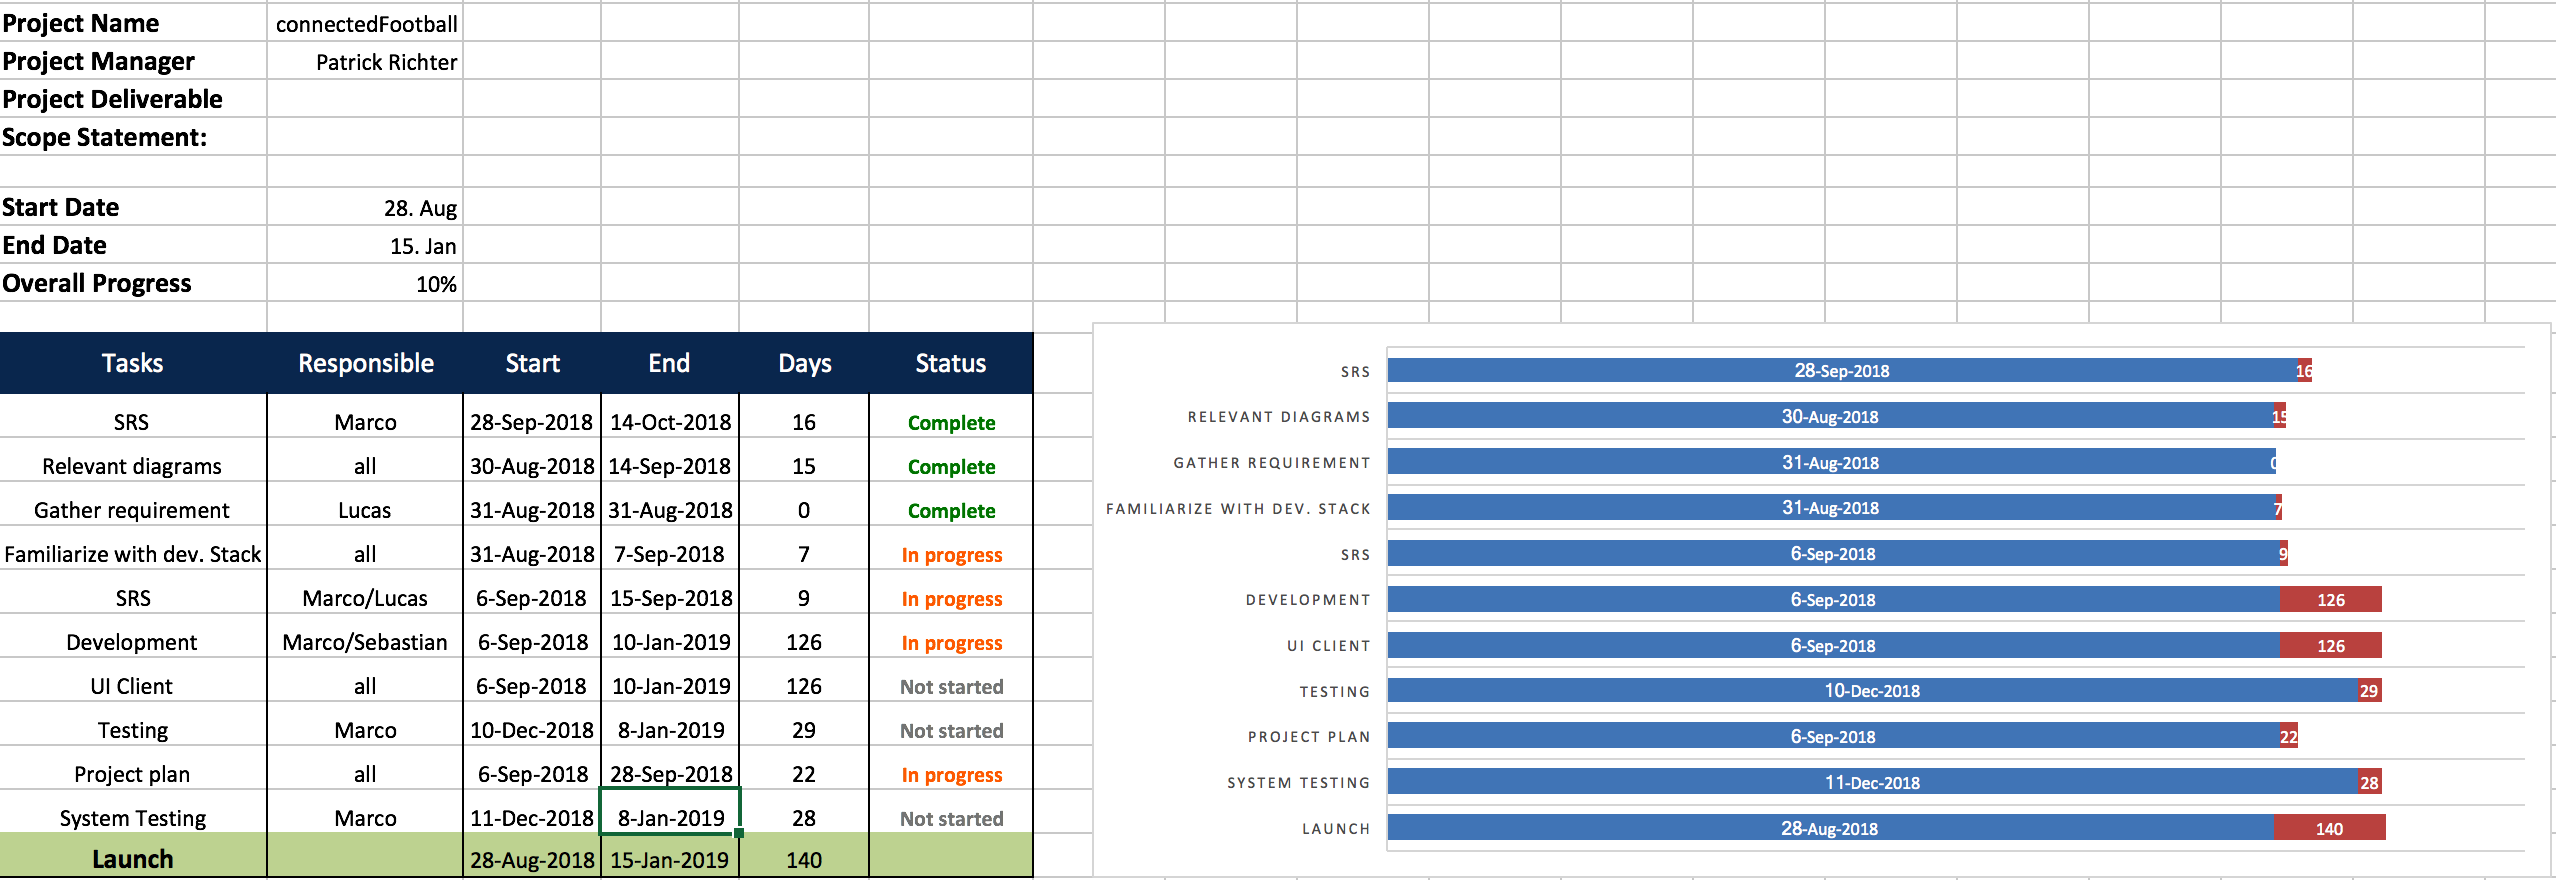
\includegraphics[width=\linewidth]{content/diagram/time/timemangement.png}
  \caption{Overview Tasks}
\end{figure}
On the right side we see a blue line with the activities. The numbers at the end of the scale with a red background are the indicated days that are needed to achieve the task. This schedule has been created at the beginning of the project and is updated continuously. 
\newpage

\subsection{Define Activities}
To get an even more detailed overview of the project tasks the activities got defined on a lower level. A \textit{Work Breakdown Structure} (WBS) was created therefore. This WBS helps to get a better overview of the single tasks. In this case everybody got assigned to every task which actually makes no sense but in the beginning of the project everybody has to work on every task, even the scrum master has to develop. Therefore, it was decided to assign everybody to every task. The development tasks got broken down in even lower level steps so the developers know exactly on what they have to work on during a sprint. Only WBS point 4 was filled completely. Over the project life cycle this information will be updated.
\begin{figure}[H]
  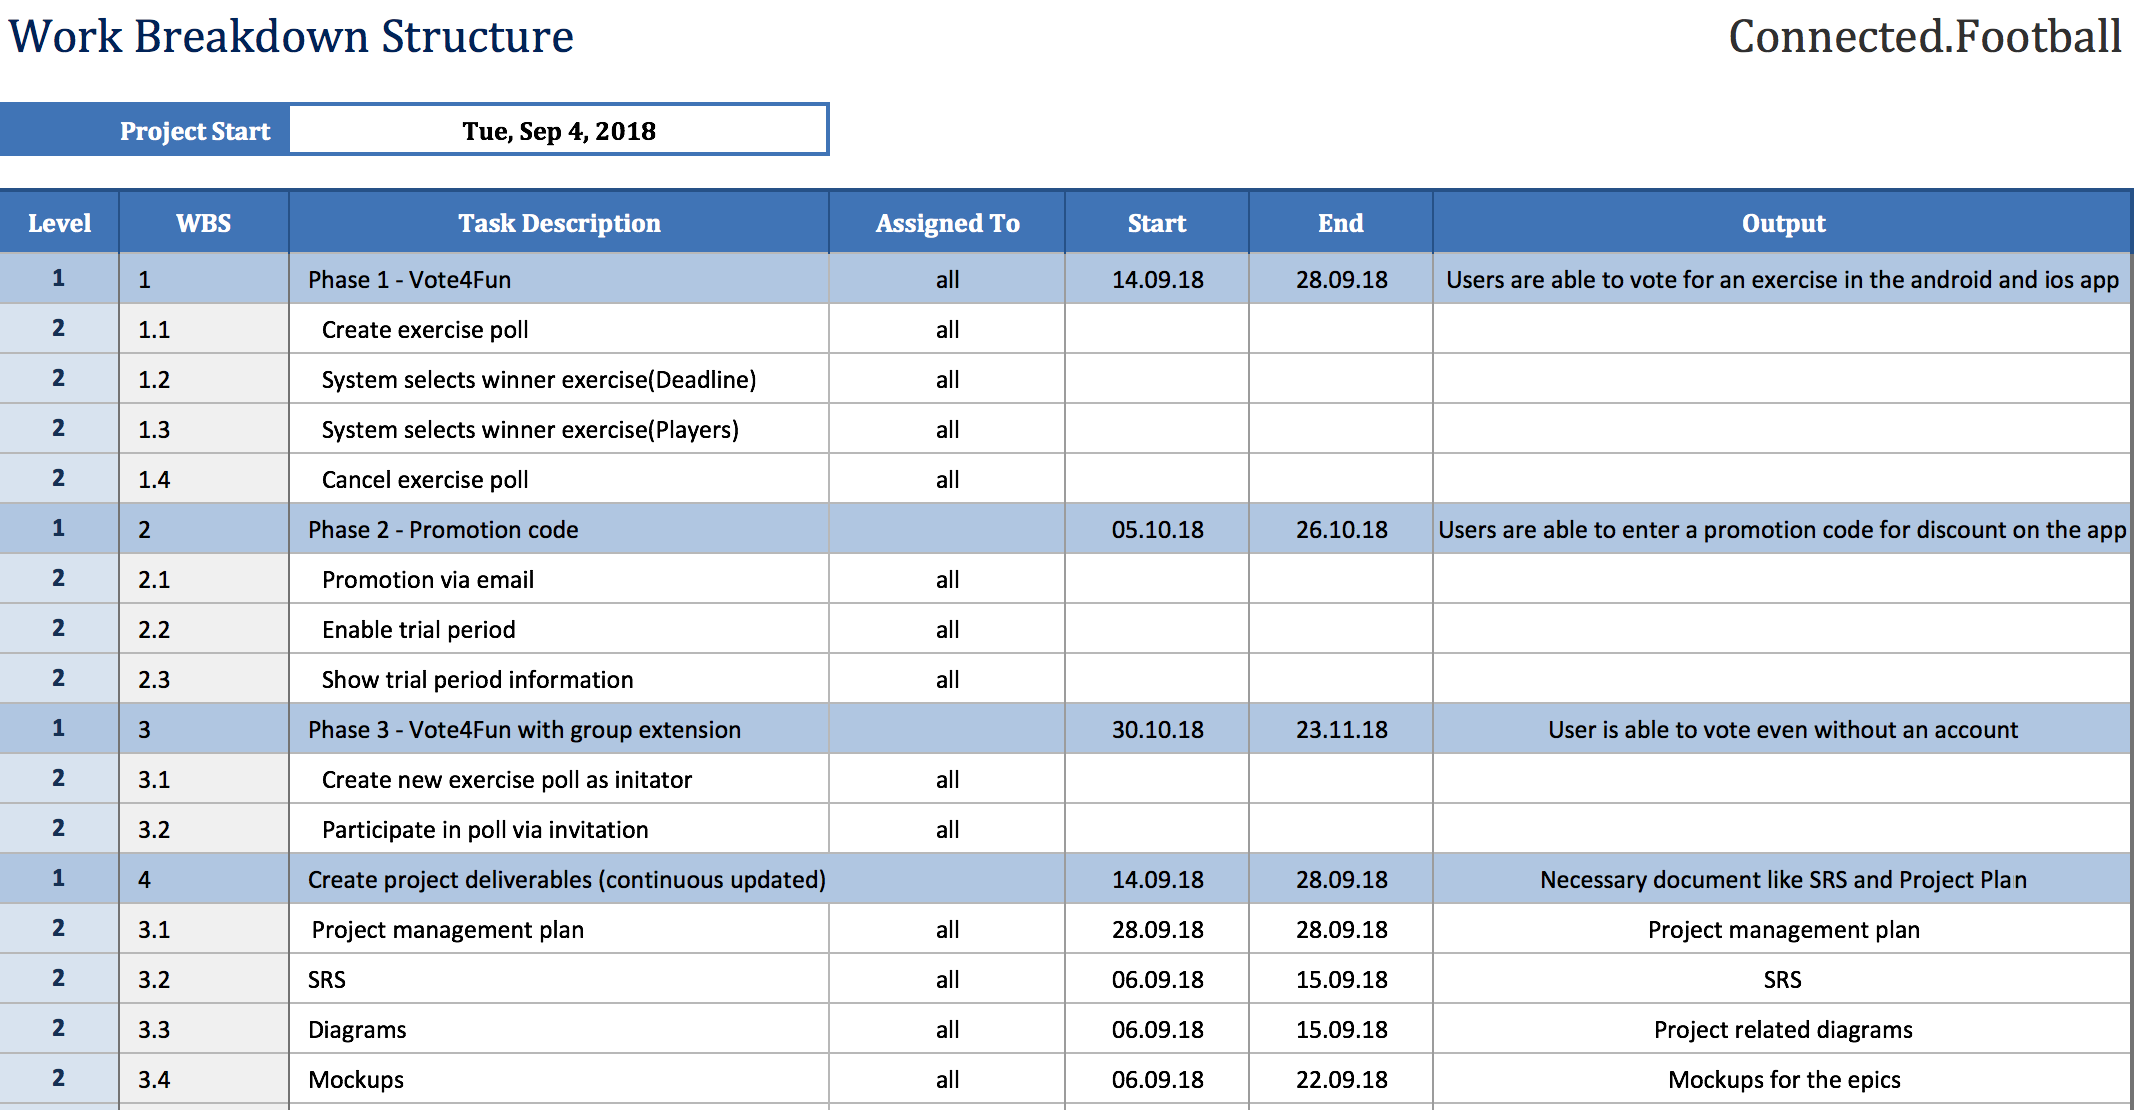
\includegraphics[width=\linewidth]{content/diagram/time/wbs_detailed.png}
  \caption{WBS detailed overview of development}
\end{figure}
What is not mentioned here is smaller sub tasks e.g. updating react-native or fixing bugs to make the app run on both devices. In particular one team member had issues making the program run on IOS which took him in total 12 hours of work ending up deploying the software on an Android device too because an activity like this consumes too much time and other more important task will suffer on completion.

\subsection{Estimate Activity Resources Process}
To achieve these activities certain resources are needed. In the project Connected.Football 4 people will work towards the success of the project. A detailed overview of the human resources and their related tasks can be found in chapter Human Resource under the chapter "Plan Human Resource Management". For a proper working environment the project members got supplied with Jira and Github accounts, further details are found in the chapter of procurement.